\chapter{實驗結果} \label{se_6}
本章節對我們實作的FaSBFT共識版本的geth 進行的測試。測試的節點皆是在Amazon EC2 t2.small上運行。t2.small 的硬體規格為1個虛擬CPU 與2GB 的記憶體。交易型態則是基本的以太坊轉帳交易。我們以交易的吞吐量Throughput(每秒共識多少筆交易量)與區塊的延遲性latency(完成一個區塊共識平均需要多少時間)與來衡量共識的效率。我們也測試共識演算法的延展性 (scalability) 以瞭解當參與共識的節點數量變多的時候,我們的共識機制的效能會受到怎樣的影響最後我們將節點分散部屬在世界各地讓該系統較貼近真實的應用場景。
\section{環境建設}\label{se_6}
所有的節點是互相連通的,即每個節點都會互相知道彼此的位置,因此我們的節點是呈現網狀連線如下圖。
\begin{figure}[H]
\centering
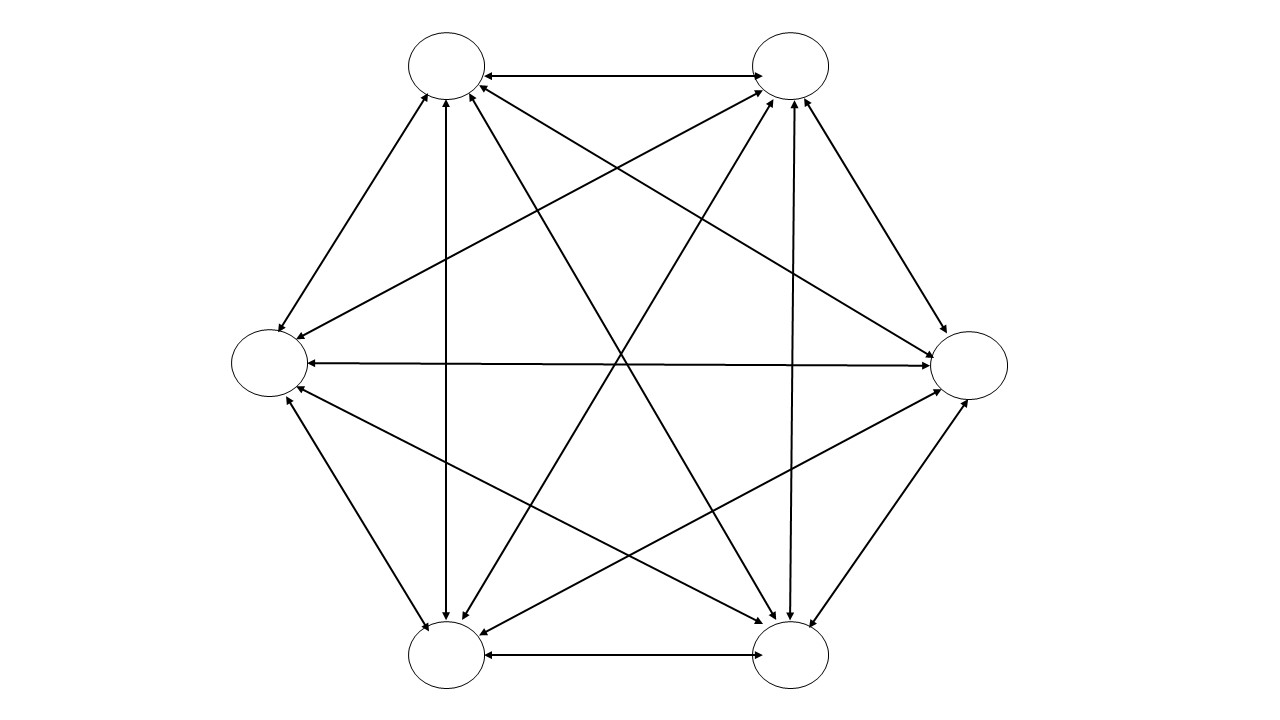
\includegraphics[scale=0.25]{images/6.jpg}
\caption{網狀連線範例圖。}
\label{i:byz-latency}
\end{figure}

%


在佈署所有節點之後,我們先讓節點互相交易約15分鐘,讓交易存入交易池內,這讓共識時產生的區塊能夠塞滿足夠的交易。
\section{同區域的吞吐量與延遲性測試}\label{se_6}
對於測試基本的交易吞吐量與延遲性測試,我們透過控制創世區塊裡的GasLimit來控制單個區塊能包含的最大交易數量,區塊大小分別為每個區塊包含500、1000、4000、8000筆交易。實驗總共進行了五種節點數分別是16、30、60、80、100 個節點。
\begin{figure}[htp]
\centering
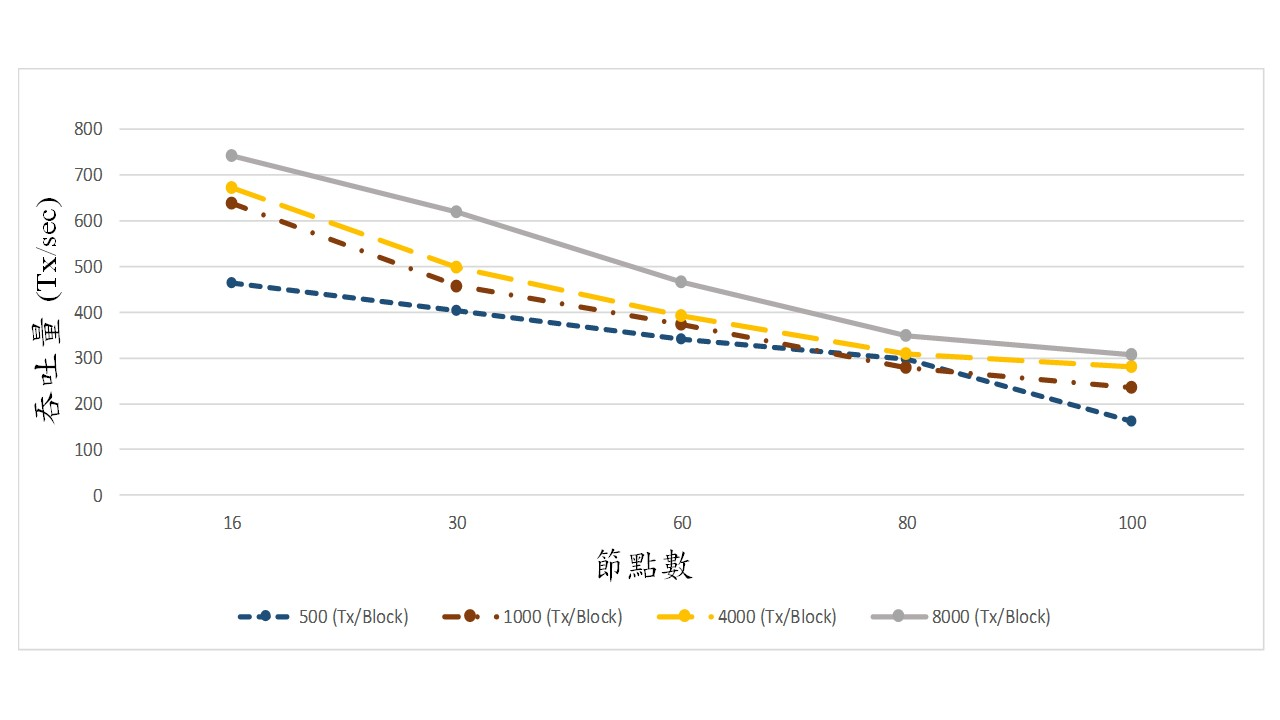
\includegraphics[scale=0.55]{images/61.png}
\caption{吞吐量 V.S 節點數}
\label{i:byz-latency}
\end{figure}
 
\newpage
\begin{figure}[h]
\centering
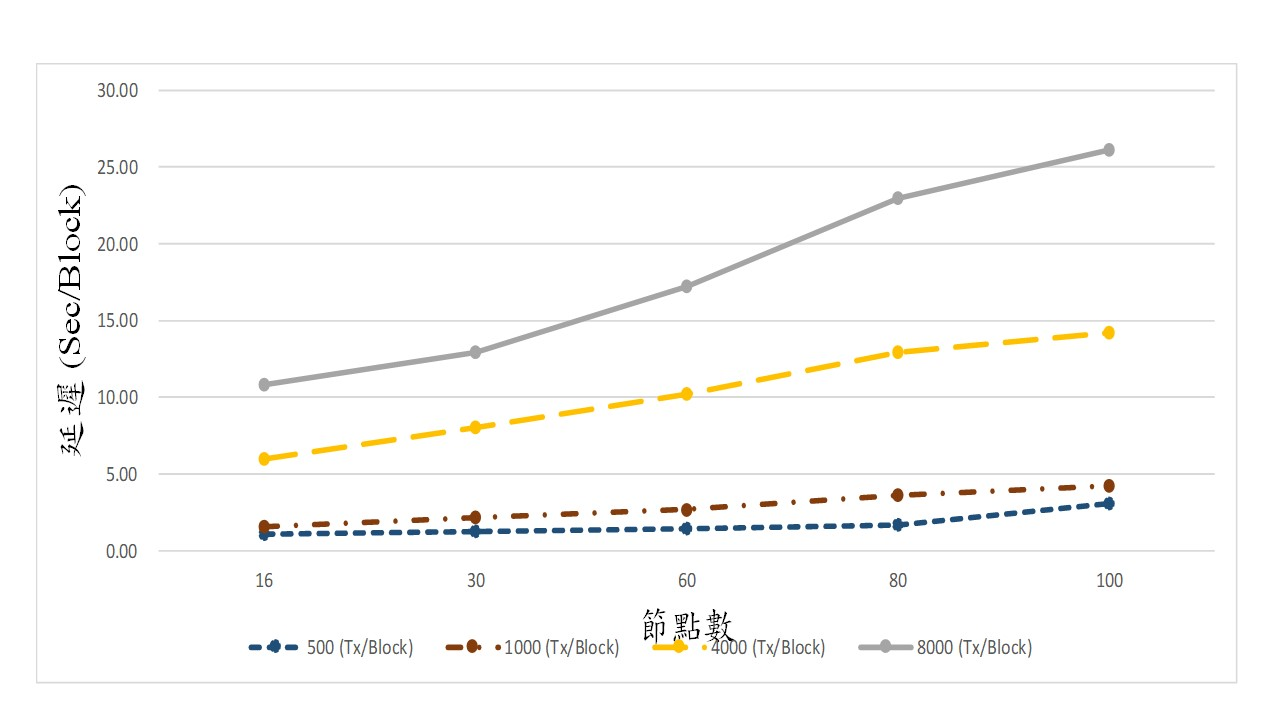
\includegraphics[scale=0.50]{images/62.jpg}
\caption{同資料中心的延遲性表現。}
\label{i:byz-latency}
\end{figure}


從圖中可以看出在我們的共識演算法在節點數增加時,共識效率會隨之下降。但當區塊大小增加時共識效率也會增加。且在100個節點吞吐量還能達到每秒300筆交易左右的共識速度,對於節點數的容忍能有良好的延展性。



\section{不同區域的吞吐量與延遲性測試}\label{se_6}
與同區域的吞吐量與延遲性測試實驗一樣,我們先讓節點互相交易約15分鐘,讓交易存入交易池內,這讓共識時產生的區塊能夠塞滿足夠的交易。區塊大小分別為每個區塊包含500、1000、4000、8000筆交易。實驗總共進行了五種節點數分別是16、30、60、80、100 個節點。不同的是我們將節點分散的部屬在世界各地。這讓實驗更加貼近真實應用。在實驗裡我們將節點平均分散在(美國-奧勒岡、美國-維吉尼亞北部、日本-東京、新加玻、倫敦)

\begin{figure}[htp]
\centering
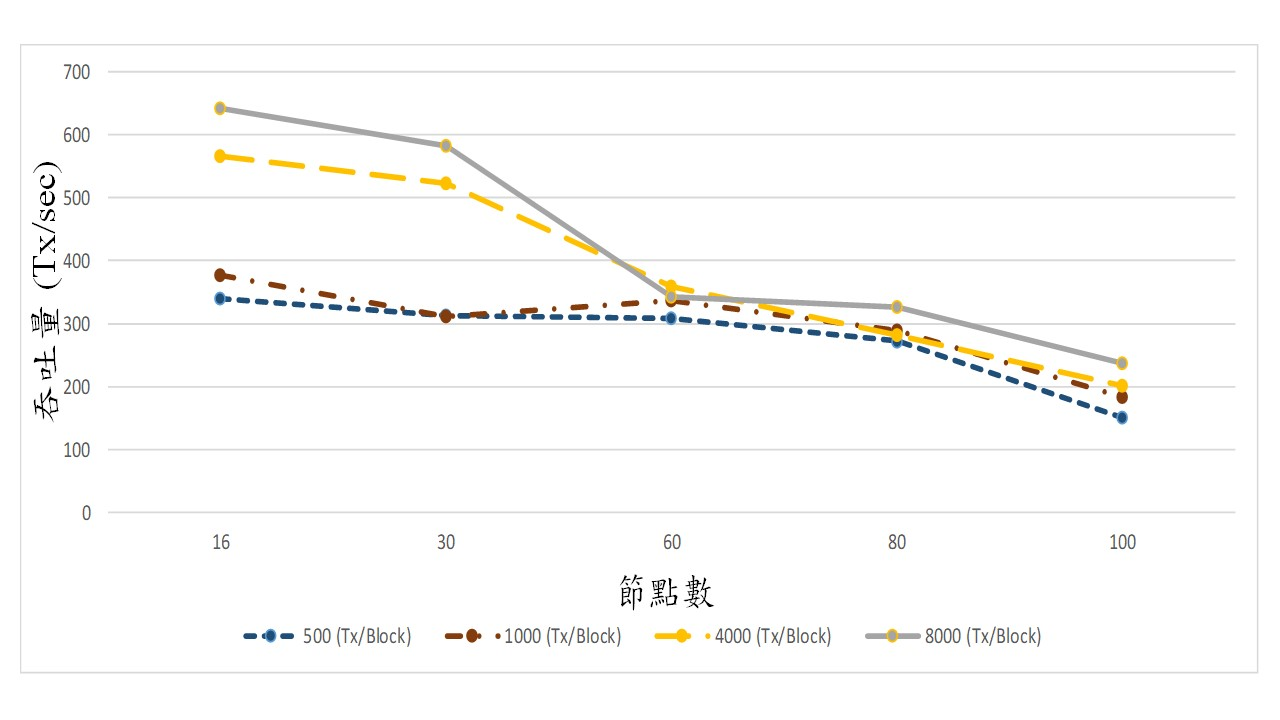
\includegraphics[scale=0.5]{images/63.jpg}
\caption{跨資料中心的交易吞吐量表現。}
\label{i:byz-latency}
\end{figure}

\begin{figure}[htp]
\centering
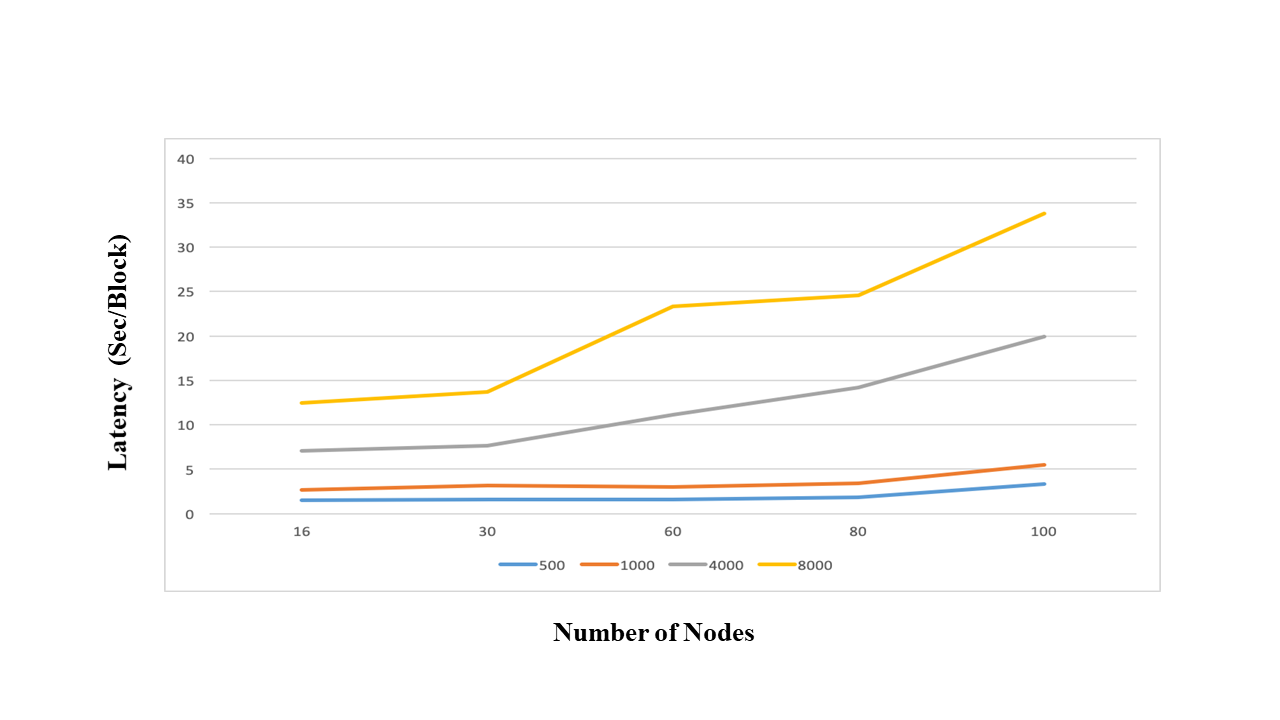
\includegraphics[scale=0.5]{images/64.jpg}
\caption{跨資料中心的延遲性表現。}
\label{i:byz-latency}
\end{figure}

%\begin{figure}[h]
{\centering
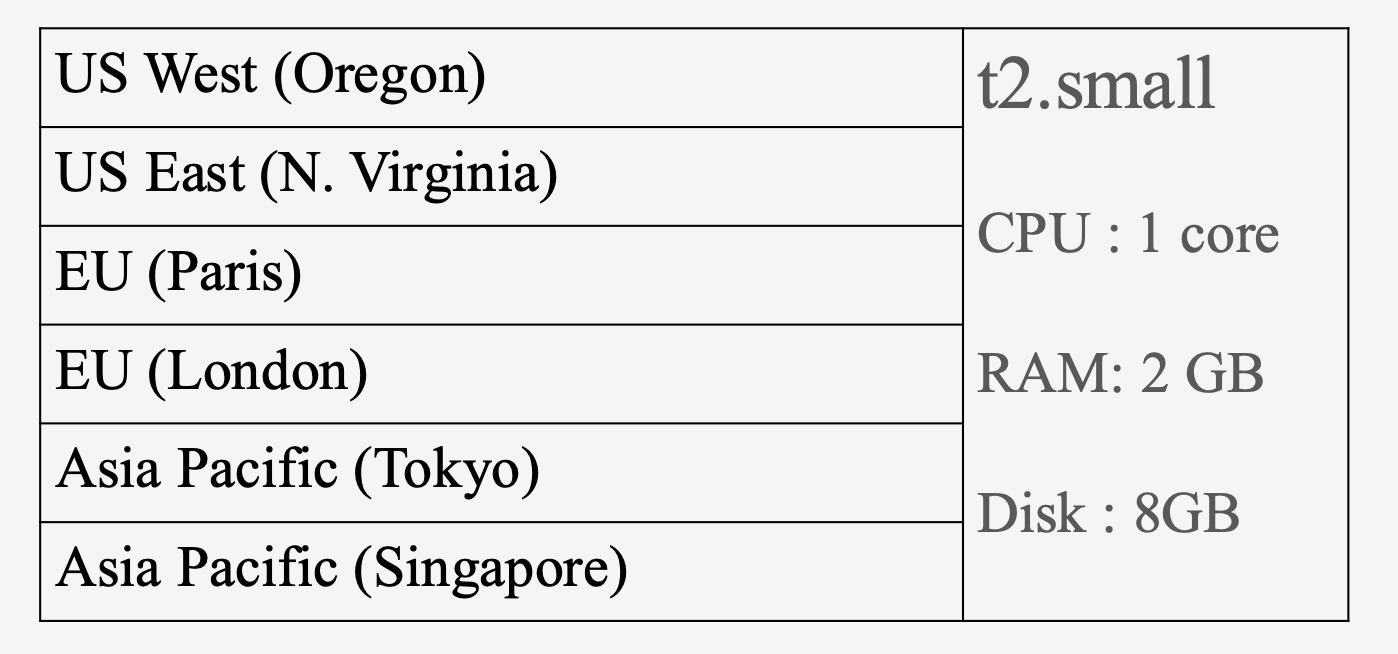
\includegraphics[scale=0.55]{images/55.png}}
\caption{實驗系統架構圖}
\label{i:byz-latency}
\end{figure}